\documentclass[letterpaper,twocolumn,12pt]{article}
\usepackage{usenix-2020-09}

% to be able to draw some self-contained figs
\usepackage{tikz}
\usepackage{amsmath}
\usepackage{hyperref}

% % inlined bib file
% \usepackage{filecontents}

% %-------------------------------------------------------------------------------
% \begin{filecontents}{\jobname.bib}
% %-------------------------------------------------------------------------------
% @Book{arpachiDusseau18:osbook,
%   author =       {Arpaci-Dusseau, Remzi H. and Arpaci-Dusseau Andrea C.},
%   title =        {Operating Systems: Three Easy Pieces},
%   publisher =    {Arpaci-Dusseau Books, LLC},
%   year =         2015,
%   edition =      {1.00},
%   note =         {\url{http://pages.cs.wisc.edu/~remzi/OSTEP/}}
% }
% @InProceedings{waldspurger02,
%   author =       {Waldspurger, Carl A.},
%   title =        {Memory resource management in {VMware ESX} server},
%   booktitle =    {USENIX Symposium on Operating System Design and
%                   Implementation (OSDI)},
%   year =         2002,
%   pages =        {181--194},
%   note =         {\url{https://www.usenix.org/legacy/event/osdi02/tech/waldspurger/waldspurger.pdf}}}
% \end{filecontents}

%-------------------------------------------------------------------------------
\begin{document}
%-------------------------------------------------------------------------------

%don't want date printed
\date{}

% make title bold and 14 pt font (Latex default is non-bold, 16 pt)
\title{\Large \bf Towards CANLay: An X-in-the-loop Virtual Testbench for In-Vehicle Security Testing with Real-time Network Performance Monitoring}

% %for single author (just remove % characters)
% \author{
% {\rm Jacob Jepson}\\
% Colorado State University
% \and
% {\rm Subhojeet Mukherjee}\\
% Colorado State University
% % copy the following lines to add more authors
% \and
% {\rm Jeremy Daily}\\
% Colorado State University
% } % end author

\maketitle

%-------------------------------------------------------------------------------
\begin{abstract}
%-------------------------------------------------------------------------------
Your abstract text goes here. Just a few facts. Whet our appetites.
Not more than 200 words, if possible, and preferably closer to 150.
\end{abstract}

% -------------- Plan ----


% --------------



\section{Introduction}
%-------------------------------------------------------------------------------
In recent years automotive security has been a much talked about topic of research. 
Researchers \cite{checkoway_comprehensive_2011} have shown that remote interfaces on modern passenger vehicles can be used to intrude into the in-vehicle network of embedded controllers, also referred to as Electronic Control Units (ECU). 
MHD vehicles expose similar interfaces that can be used to control/disrupt critical functions \cite{mukherjee_practical_2016,burakova_truck_2016} typically operated by ECUs using sensors and actuators. 
To evaluate the effectiveness of their approaches, researchers have traditionally experimented on real-vehicles or homegrown testbed setups that mimic real vehicles. 
While most households in the United States have at least one passenger car\footnote{\url{https://www.statista.com/statistics/551403/number-of-vehicles-per-household-in-the-united-states/}}, this is not the same for medium and heavy-duty (MHD) vehicles. 
Moreover, creating homegrown testbeds is both logistically and economically challenging. To that end, the need for a publicly accessible testbench is imminent.

% The first criteria to this type of testbed is accessibility the ease with each the testbench can be accessed. 
There are two important criteria that reseach in this area has established for this type of testbench. The first is fidelity, i.e. the ability of the setup to replicate a real-world in-vehicle networking infrastructure. The second is adapability i.e. the ability to be reconfigured to suit different needs. It may be difficult to maximixe the extent to which both these criteria is achieved. The most adaptible testbed is the one in which ECUs as well as the network  configuration can be programmed on the fly. Existing solutions have enabled ECU virtualization but not network virtualization for real-world ECUs. In those setups, ECUs from different physical locations cannot be used in the same testbed, neither can networks be configured on demand, unless the ECU is virtualized.
We believe that having real-world ECUs in the testing setup is critical. This not only provides greater fidelity but also alleviates any concerns with intellectual privacy and availability on the ECUs. Another aspect to fidelity and adaptibility is the realization of vehicular conquality of the network 
Existing solutions 

In this 

% The problem of remotely accessible testbeds for automotive control systems has been addressed in the past \cite{tagarev_automotive_2021}. A recent survey on the same identified an issue with the adaptability, i.e. the ability to adapt to user demanded configurations. Of the testbeds covered in \cite{tagarev_automotive_2021} and the only effective solution is a portable hardware testbench, PASTA \cite{}. There are two ways to adaptibility, virtualizing the ECU and/or virtaulizeing the network configuration. Most existing solutions have suggested virtualizing the ECU by reprograming the hardware to user demands. While this is viable solution, To achieve both, existing techniques have used a full virtualization scheme. 

\section{Design Goals}
\begin{figure}[t!]
    \centering
    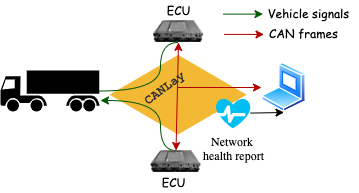
\includegraphics[width=\linewidth]{images/design_goal.drawio.png}
    \caption{Design Goal of CANLay}
    \label{fig:goal}
\end{figure}
% The overarching design goal of this project is eludiated through figure \ref{fig:goal}. In summary, our goal is to create an overlay over TCP/IP that can transport CAN frames and vehicle control signals to ECUs located in different subnets accross the globe. The control signals can be obtained from and fed back into a vehicle simulator that is the under the user's control. 
% The simulator is expoted to be useful in controlling the sensory inputs to the ECUs as well realize the effect of actuation. The overlay is expected to serve two purposes: create user demanded network configurations and make use of ECUs from different physical locations, possibly crowsourced. This model is designed in light of the software defined truck paradigm introduced in \cite{mukherjee_towards_2021}. In pursuit of the above mentinoned design goals, we identified four tasks. These task, along with the associated challenges, are described next. 

% \paragraph{Overlay Connection Management}
% \paragraph{Facilitation of CAN Data Manipulation via Vehicle Control}
% \paragraph{Facilitation of Vehicle Control via CAN Data Manipulation}
% \paragraph{Enabling Crowdsourcing of ECUs}



\section{Design}
\begin{figure*}[t!]
    \centering
    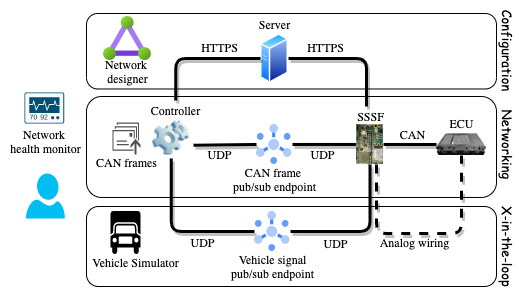
\includegraphics[width=\linewidth]{images/system_design.drawio.png}
    \caption{Proposed System}
    \label{fig:goal}
\end{figure*}

\subsection{Current Status of Development}

\subsection{Component Descriptions}
\subsubsection{Smart Sensor Simulator and Forwarder (SSSF)}
The Smart Sensor Simulator and Forwarder (SSSF) emulates the electronic systems of a truck. By emulating the required sensors of a truck, it eliminates many of the unnecessary error messages that would normally indicate that a component is missing. In turn this allows the operator to communicate with the ECU as if it was in normal operating conditions. Having the ECU believe it is in normal operating conditions is necessary to use the ECU in a test bed setup. 

Furthermore the Smart Sensor Simulator and Forwarder acts as a gateway enabling the ECU to access and more importantly, to be accessed by, the CANLay system. The SSSF is equipped with an Ethernet port allowing it to communicate with the CANLay system via the Internet. When an SSSF is being used in an active session, it acts as a forwarder between the controller and the ECU. The SSSFs are responsible for forwarding 2 types of messages. The first type is sensor messages from CARLA in which the SSSF applies any necessary transformations to the sensor messages and forwards them to the ECU. The second type of message is CAN messages both from their respective ECUs and from other SSSFs in the current session. In other words the SSSF forwards CAN messages it receives from its ECU to the other devices and forwards CAN messages from the other devices to its ECU. This allows multiple ECUs to actively communicate with each other in a session, creating a richer testing environment.

\subsubsection{Controller}
The Controller acts as a user interface to the CANLay system and enables vehicle simulators to communicate with the CANLay network. The Controller’s user interface is used to assist the user in building their virtual test bed. It does so by informing the user of the available ECUs, recording the choices, and communicating the desired network nodes with the central server. Once the session setup is completed the controller transitions to acting as a gateway for a graphical vehicle simulator to communicate bi-directionally with the CANLay system. In a similar fashion to the SSSF the Controller forwards in-game signals to the multicast endpoint and listens for CAN messages from the multicast endpoint. Overall the Controller acts as the means of control for the virtual test bed.

\subsubsection{Server}
The server acts as the broker in a publisher subscriber model. Each device opens and must maintain a persistent TCP connection with the server while they participate in the CANLay system. Once the TCP connection is established the devices communicate with the server through HTTP APIs. The server acts as the coordinator between the Controllers and the SSSFs. This allows the server to monitor the health of the devices and take actions if a device is malfunctioning or goes offline. It also allows the server to keep track of free devices and free multicast endpoints so it can properly validate new session requests and allocate the requested devices and endpoints without running into race conditions or double use issues that may arise if each Controller was in charge of allocating its own session. Finally, the server keeps track of ongoing sessions and ensures the proper closure of a session in the event a device is experiencing issues.

\subsubsection{Vehicle Simulator}
The Vehicle Simulator is any software that provides the user with the ability to control a vehicle in a digital world. To be compatible with the CANLay framework the Vehicle Simulator must expose its in-game vehicle operating signals in some manner. For the purpose of this paper we chose the graphical vehicle simulator called Carla. Although the Carla project mainly focuses on autonomous driving research it was chosen for this paper because it exposes its in-game signals through an easy to use python api. In addition the Carla project pays close attention to the scientific details represented in its simulator. While this is not required, the more realistic and accurate the signals are, the easier it will be to transform them into CAN messages. Furthermore, it is not required that the vehicle simulator have a graphical component or be controllable by the user, but we suspect they will be integral to the prevailing way in which the CANLay framework is used.

\subsubsection{Publish/Subscribe Endpoints}
The publish/subscribe messaging mechanism is “a form of asynchronous service-to-service communication” where “any message published to a topic is immediately received by all of the subscribers to the topic.” (cite https://aws.amazon.com/pub-sub-messaging/) The publish/subscribe mechanism used in the CANLay framework is UDP multicast. Therefore, a pub/sub endpoint in the CANLay network is a multicast address and port pair. Although the CAN frame and Vehicle signal pub/sub endpoints are shown separately in the above diagram for clarity, they are physically a single endpoint in the network. The pub/sub model was chosen because it is similar to a CAN network in that an ECU is “subscribed” to all other ECUs on the same CAN bus and all other ECUs on that CAN bus are subscribed to that ECU. This form of total participation pub/sub model is also very similar to a broadcast mechanism. The only difference between a publish/subscribe model and a broadcast model is the use of one or more brokers which control which nodes are able to subscribe to each other. 

In order to find a publisher subscriber mechanism that closely resembled that of a CAN network we defined these criteria. The first requirement is that the transport mechanism must support some form of message broadcasting which enables a sender to send one message that can be received by many receivers. This requirement is important because the number of connections the sender will need to manage will stay constant no matter the number of devices in a group. In turn this keeps the sending time of a message at O(1) instead of O(n). The next requirement is that the transport mechanism must enable the devices to receive messages from one or more devices while having to maintain only one connection. In addition the transport mechanism must not have any implicit congestion control or flow control since none is found in CAN networks. Finally, it's preferable if the communication mechanism transported data as individual messages rather than streams of data.

UDP multicast was found to be a suitable local network transport mechanism that satisfied the above requirements. We note that while UDP multicast is suitable for use within an autonomous system it may not be a suitable publisher subscriber mechanism for use between autonomous systems. As a result we are exploring other potential models such as MQTT.

\subsubsection{User Interface to CAN}
Upon arrival at the controller CAN messages can be interpreted and applied as transformations to the in-game vehicle signals, recorded and saved, or forwarded to a local VCAN endpoint. Interpreting CAN messages and applying their transformations to in-games signals provides visual feedback to the operator about actions ECUs are attempting to perform. Unfortunately generalizing specific CAN messages is much more challenging compared to specializing signals messages from the game. As such it currently provides little to no scientific value. As an alternative to evaluating the test using visual feedback from the game, the CAN messages can be recorded and analyzed after the test has completed. Finally, if the user would rather work with the CAN messages using socketcan tools, the messages can instead be forwarded to a VCAN endpoint.
    
We haven't implemented the transformation or the VCAN stuff yet so idk if it should go in the paper.

\subsubsection{Network health monitor}
A large drawback of connecting devices over a shared/multipurpose network is the increase of networking delays. When a user creates a virtual test bed using CARLay they are logically forming a virtual network for that session, but physically each device is still connected to the same network as before. As a result, communication between devices in a virtual test bed could suffer from network delays that are out of the user’s control. The Network Health Monitor provides the user with useful information about the current status of the network so they can ensure that the current network conditions are not affecting their results. The network information is gathered from the perspective of all devices in a session rather than collecting it from just the perspective of the Controller. This provides a more full view of the current state of the network.

\subsection{Behavior Descriptions}
\begin{figure}[t!]
    \centering
    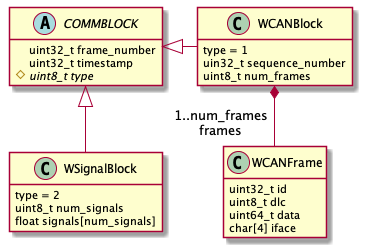
\includegraphics[width=\linewidth]{out/images/data_structures/data_structures.png}
    \caption{}
    \label{fig:}
\end{figure}

\subsubsection{Overlay Setup}
A typical setup of the CANLay system begins by first starting up the central server. Once started the central server can begin accepting HTTP API calls. HTTP API calls were chosen because they clearly define the object to invoke and the manner in which to invoke it. The HTTP Uniform Resource Indicator (URI) is used to distinguish the object or api endpoint to be invoked. At the top level the Server has two main api endpoints namely “\\Controller” and “\\SSSF”. Nested underneath each of these endpoints are the endpoints “\\Register” and “\\Session”. The “\\Register” endpoint is used to control the registration of the connected device and the “\\Session” endpoint is used to control the session associated with the connected device. The HTTP method is used to describe the manner in which to invoke the api endpoint. Typically “GET” is used to gather information, “POST” or “PUT” are used to supply information, and “DELETE” is used to remove information. Examples of these HTTP API calls will be shown throughout the paper. (Also the http api description doesn’t seem like it belongs here but I feel like it is important for the reader to understand how a device actually registers or starts a session)

Once the server is up and running we can begin connecting devices to it. Usually the first device to connect to the server will be an SSSF. The SSSF starts by reading the SD card connected to it. This SD card describes the devices attached to the SSSF since there is currently no reliable way to detect the type, year, make, model, and serial number of the connected ECUs via only CAN messages. Next the SSSF gathers its MAC address and list of attached devices into a JSON and sends it to the server via a POST to the HTTP API endpoint “\\SSSF\\Register”. The server will parse and validate the registration. If the registration is satisfactory, it will reply with a code 202 indicating to the SSSF that it has successfully registered with the server. If the registration is not satisfactory such as a duplicate registration, invalid attached device, or invalid JSON the server will respond with the appropriate error code and drop the connection. If the SSSF successfully registered it will wait for further instruction from the server. In the meantime the SSSF will begin the processes of synchronizing its Real Time Clock using NTP.

Next a Controller may connect to the server. The Controller will first begin by registering with the Server in a similar manner to the SSSF except that the Controller has no attached devices so it will only send its MAC address to the endpoint “\\Controller\\Register”. The server will once again parse and validate the registration and respond with the appropriate code. If the Controller successfully registered then it proceeds to make a “GET” to the HTTP API endpoint “\\SSSF”. This asked the server for a list of all of the available SSSF devices. Please note that if a SSSF device is currently being used in another session it is not considered available. After the controller has received the list of available devices it presents the available ECUs to the user. Notice that while the Server deals with the SSSF devices a user will typically only be interested in the ECUs that the SSSF is acting as a gateway for. After the user finalizes their selection the Controller will make a “POST” containing the selected devices to “\\Controller\\Session”.

When the server receives a session request it first checks to make sure that the request is coming from a registered Controller. Next the server confirms that the devices are still available. If any of the devices are no longer available or become unavailable during the session setup process, the server responds to the Controller with the error code 409 indicating there's a conflict in the selection. If the Controller receives this message it will start the session selection processes over again. If all of the devices are still available the Server then selects an available multicast endpoint for the session and assigns an index to each device. The index is used in the collection of network statistics which will be explained later on. Now the server begins notifying the devices by sending a “POST” to the device’s root URI (“.”) containing the unique ID and index of the device, the selected multicast IP and port, and a list containing the ID and attached devices of other nodes in the session. Finally once all SSSFs have been successfully notified the Server response back to the Controller with the same session information it sent to the other devices.

Once any device receives a session setup message it will parse and validate the request and respond to the server accordingly. If a session setup message checks out then it will shorten its NTP polling interval, allocate space for the required data structures, and begin listening for and forwarding messages to and from the multicast endpoint. At this point the session setup is completed.

% \begin{figure}[t!]
%     \centering
%     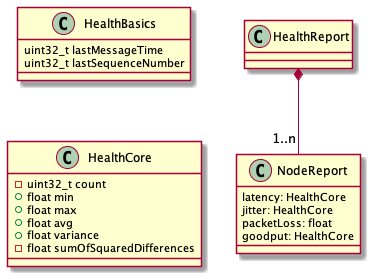
\includegraphics[width=\linewidth]{out/images/network_health/network_health.png}
%     \caption{}
%     \label{fig:}
% \end{figure}
\subsubsection{X-in-the-loop Simulation}
\begin{figure}[t!]
    \centering
    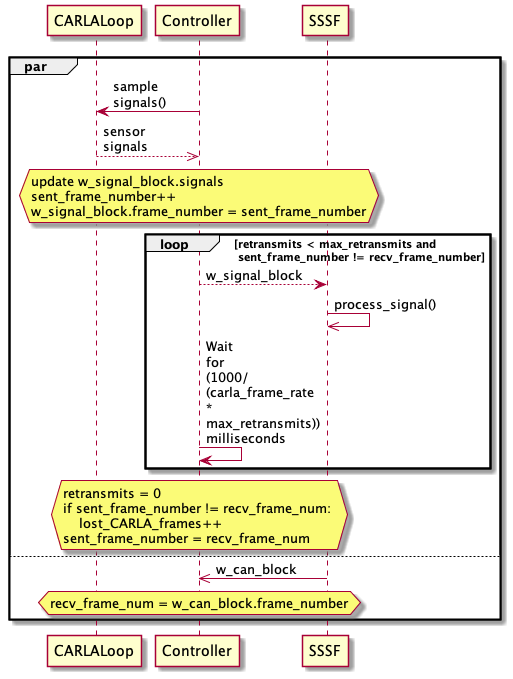
\includegraphics[width=\linewidth]{out/images/signal_control/signal_control.png}
    \caption{}
    \label{fig:}
\end{figure}
\subsubsection{CAN communication}
\begin{figure}[t!]
    \centering
    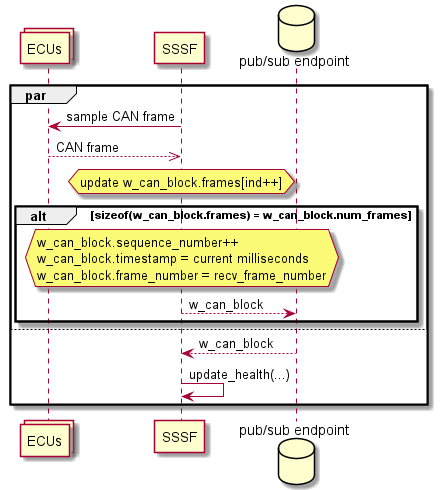
\includegraphics[width=\linewidth]{out/images/can_exchange/can_exchange.png}
    \caption{}
    \label{fig:}
\end{figure}
In order to create a virtual test bench of ECUs the devices must be able to communicate with each other as if they were talking via a CAN bus. Most ECUs do not come with built in ethernet ports and the ability to broadcast CAN frames via Ethernet. So in order to connect an ECU to Ethernet we need a device that can interface with a CAN network and interface with an Ethernet Network. This is why the Smart Sensor Simulator and Forwarder is necessary. It acts as a programmable gateway that can transfer messages between the CAN network and the Ethernet Network.

When the SSSF is in an active session it first checks if one or both of its CAN networks were assigned baud rates. If the CAN network was assigned a baud rate, it attempts to read a message from the CAN network. If it reads a message from the CAN network, it proceeds to create the COMMBlock message that will be written to the CANLay network. The COMMBlock message requires some additional information before it can be written to the network. First a type ID is added which indicates the type of message the COMMBlock is carrying. In this case the type will be 1, indicating that it is carrying a CAN message. It will also need to add the current millisecond timestamp at which it is sending the message. This is used by other devices to calculate the network latency for the network path from this device. Also, a sequence number is added and incremented every time a CAN message is sent. If other devices on the network detect gaps in the sequence numbers they know that a message has been lost. In addition it will also append the frame number of the last frame it received from the Controller. If it has not received any frames from the Controller then this number will be zero. The last seen frame number indicates to the Controller which SSSFs have and have not received the last sent frame. Also, the SSSF will mark whether this CAN message is a canFD CAN frame. Finally, the SSSF will mark whether or not this message requires a response. The CAN message requires a response if its CAN frame’s PGN matches a list received from the user.

After the SSSF is done checking for CAN messages from the CAN network, it moves on to check for messages from the multicast network. Again, CAN messages sent to the multicast endpoint are considered type 1 messages. So if an SSSF device receives a type 1 message it first checks if the message requires a response. If so, it replies to the multicast endpoint with a type 5 message with the frame number equal to the sequence number of the message it just received. Next it updates its network statistics about the device it came from using the sequence number, timestamp, and other metrics from the COMMBlock and then it writes the FlexCAN CAN frame onto its available CAN networks.
% This is supposed to be sudo code btw
    if (msg.type == 1)
    {
        if (msg.needsResponse)
        {
            writeToMcastEndpoint(5. msg.sequenceNumber);
        }
        networkHealth->update(msg);
        if (can0BaudRate) can0.write(msg.canFrame.can);
        if (can1BaudRate) can1.write(msg.canFrame.can);
    }

\subsubsection{Network health monitoring}
\begin{figure}[t!]
    \centering
    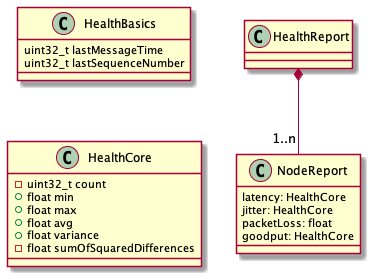
\includegraphics[width=\linewidth]{out/images/network_health/network_health.png}
    \caption{}
    \label{fig:}
\end{figure}
As discussed earlier, monitoring the health of the network is key to ensuring that bad delays or large amounts of packet loss are not affecting your test results. In order to enable the devices to collect network statistics during an active session, each message is loaded with additional information. The first piece of additional information is a frame number. The Controller increments the frame number everytime it sends out new signals. When the SSSFs receive a message with a frame number higher than the previous frame number they saw, they send their frame number to the new frame number. Whenever SSSF devices send a message they add that frame number to the top of it. Therefore when a Controller receives a CAN message it can check the last frame the device had received when it sent the CAN message by checking the frame number in the COMMBlock. This system enables acknowledgement of messages without having to send any additional messages. In addition if an SSSF spots a gap in the frame numbers that is larger than 1, then it knows that a frame has been lost.

The type 1 COMMBlock messages (messages containing CAN frames) include a sequence number in addition to the frame number discussed earlier. Whenever an SSSF device sends out a CAN message, it adds a sequence number and increments it by 1. Signals from the controller are sent at the frame rate of the game. This means that with a frame rate of 60fps the Controller is sending messages about 3-4x slower than the message rate seen in on a 250,000 baud ECU operating at nominal bus load. As such we cannot expect the acknowledgement mechanism used for the Controller messages to work for the CAN messages. However other devices can still use the sequence numbers to detect dropped CAN messages by looking for gaps larger than 1.

The next important metric included in the COMMBlock messages is a timestamp. Timestamp is included to allow devices to calculate the latency along the network edge from the sending device to the receiving device. Of course this could be done by performing network tests during an active session but unless the latency is guaranteed to always be low, this testing could interrupt the normal flow of the other messages being sent in the session. So instead the timestamp is included with each message that is sent so that network health metrics can be calculated on the fly and performed without interrupting the testing. The latency is calculated by subtracting the time at which the message was sent from the time at which the message was received. The downside to this method is that it requires all of the device's clocks to be synchronized as close as possible. With the current basic implementation of the NTP protocol, the devices on average stay within a millisecond or two of each other when they are all referencing an NTP server on the same network. Unfortunately when the devices use different NTP servers that are much farther away the devices tend to stray between 5-15 milliseconds from each other. This creates issues when trying to measure the latency of devices that are very close to each other. It's important to note that more advanced implementations of NTP may be able to shrink these numbers.

Overall, these indicators enable each device to calculate four network statistics for every other device on the network namely packet loss, latency, jitter, and goodput. Packet loss is the number of packets determined to be lost along a network edge. Latency is the time it takes for a message to go from the sender to its receiver. Jitter is the variance in latency. There are many different types of network jitter but we use the simplest form which is often called packet jitter or constant jitter which is defined as “packet jitter or packet delay variation (PDV) is the variation in latency as measured in the variability over time of the end-to-end delay across a network” (cite https://networkencyclopedia.com/jitter/). Goodput is the measurement of application level throughput. In our case it is calculated in bytes per second.

Every second the Controller sends out a type 3 message which requests the health report from each device. After each device has sent their health report to the Controller they reset their statistics, keeping only the last message timestamp and the last seen sequence number. This effectively creates a measurement period of 1 second. As the Controller receives the health reports, it updates the network statistic data structure and displays the new results to the user. By collecting health reports from each network node we are able to get the statistics about a network edge from devices on each side of that network edge (how do I explain the importance of the network stats matrix better?).


\section{Analysis}


%-------------------------------------------------------------------------------
\bibliographystyle{plain}
\bibliography{bib}

%%%%%%%%%%%%%%%%%%%%%%%%%%%%%%%%%%%%%%%%%%%%%%%%%%%%%%%%%%%%%%%%%%%%%%%%%%%%%%%%
\end{document}
%%%%%%%%%%%%%%%%%%%%%%%%%%%%%%%%%%%%%%%%%%%%%%%%%%%%%%%%%%%%%%%%%%%%%%%%
